\documentclass[conference]{IEEEtran}
\IEEEoverridecommandlockouts
% The preceding line is only needed to identify funding in the first footnote. If that is unneeded, please comment it out.
\usepackage{cite}
\usepackage{amsmath,amssymb,amsfonts}
\usepackage{algorithmic}
\usepackage{graphicx}
\graphicspath{{figures/}}
\usepackage{textcomp}
\usepackage{xcolor}
\usepackage{balance}
\usepackage{url}
\def\UrlBreaks{\do\/\do-}
\def\BibTeX{{\rm B\kern-.05em{\sc i\kern-.025em b}\kern-.08em
    T\kern-.1667em\lower.7ex\hbox{E}\kern-.125emX}}
\begin{document}

\title{The Evolution of German Rap Lyrics}


\author{\IEEEauthorblockN{Luca Schumann}
\IEEEauthorblockA{\textit{lucsc442} \\
\textit{TDDE16}}
}

\maketitle

\begin{abstract}
Test
\end{abstract}

\section{Introduction}
Introduce the task or research question that you have addressed in
your project. What were you trying to do? Why did you choose this project?

\section{Theory}
Present relevant theoretical background, and in particular the models that
you have used. Where appropriate, use mathematical formulas.

\section{Data}
Present your data. What information does it contain? Where did you get it
from? What preprocessing did you do, if any?

\subsection{Dataset}
First of all, a selection of songs had to be made. To find a balance between relevant artists in the CD era and the streaming era, I decided to combine lists of artists from two sources. I selected all 46 german artists from the Wikipedia list of Rappers that sold more than 100,000 albums in Germany \cite{wiki_albums}. The popularity of musicians today, especially Rappers, is not only defined by the albums sales but also the online streams. Therefore I picked all 13 Rappers appearing in the Spotify playlist "Top German Artists of 2020" \cite{spotify_2020} that were not in the selection yet. To increase the dataset, I chose 18 more objectively popular Rappers, adding up to 77 artists in the end.\\
The lyrics of the artists' songs were then downloaded using the Genius API \cite{genius} with help of the \textit{lyricsgenius}package \cite{lyricsgenius}. A lot of the songs are duplicates, since remixes, features and live versions are all included in the genius database. There are furthermore many non-songs in the database, such as commentaries. Luckily, most could easily be ignored by discarding songs that contain brackets, as in \textit{Papa ist da (AsadJohn Remix)}. Few others had to be handled differently, but the final dataset is clean of such occurences. In a first run of the model, songs containing english lyrics formed an individual topic. Upon manual inspection, there were a few songs with parts in english, or even completely in english. Therefore, songs that contain all the most common english words in the english topic "the", "you" and "and" were suspected to contain english lyrics and also discarded. The final dataset features almost 7500 songs.

\subsection{Preprocessing} \label{preprocessing}
Preprocessing the song lyrics was an iterative process with many learned lessons. The most basic first step is to remove meta information that is written in brackets from the lyrics, such as \textit{[Hook]}. Next, the songs are tokenized using spacy's German package. Non-alphabetic tokens, stop words and tokens with less than three letters are removed. The rest of the preprocessing is done with Gensim. Bigrams and Trigrams are added and extremes are filtered. Finding the seemingly best values for these tasks was done with the trial and error method.\\
After excluding english songs from the dataset, the model would still find a topic with mostly english stop words. After removing english stop words during preprocessing, the problem was solved. Another problem was many artist's names appearing in the most salient words of some topics. The reason for this is that some Rappers are notorious for talking and singing about themselves in the third person. Rappers with a lot of songs in the dataset would therefore skew the results, although their own name has nothing to do with the message behind their song. To tackle the problem, each artists name was removed from his or her lyrics. Unfortunately this method is not foolproof, as some refer to themselves by nicknames, e.g. \textit{Ufo361} simply calling himself Ufo. As a final tweak of the preprocessing step, a couple of stop words that were not in spacy's German list were manually removed.\\
Tokenizing German text turned out to be a difficult task, with no really satisfying solution. In German texts, all nouns are capitalized, therefore also in spacy's word list. If a word at the beginning of a sentence is capitalized, it is not possible for spacy to tell wether it's a noun or not. Feeding spacy all words in lowercase would also not solve the problem, since it would not recognize the nouns anymore. Additionally, some words have a different meaning depending on wether they are a noun (capitalized) or not. E.g. "Weg" means path but "weg" means away in German. This appears to be an unsolved problem as of today, as can be read on spacy's Github forum \cite{spacy_issues}. Lemmatization does also not work as well as for english text, but overall the results are good enough to work with them.

\section{Method}
Explain how you carried out your study. Aim to be detailed enough for
others to reproduce your results.

\section{Results} \label{results}
Present your results in an objective way. Use tables and charts, but do not
forget to also include a summary in text form. Do not interpret your results

\subsection{The Topics}
The final iteration of the model found five topics that I named "Street", "Sex \& Party", "Love \& Life", "Competition" and "Lifestyle". Table \ref{tab:topics} shows the eleven most salient terms for each topic, translated to English. It strucks right away that many English terms are used in the lyrics, especially in the "Lifestyle" topic, were seven words are not translated. Interestingly, there are none in "Street" or "Love \& Life". Some words such as \textit{see}, \textit{man} or \textit{yeah} make it in the top terms of multiple categories. \textit{Come} for example even appears twice very high up in the "Sex \& Party" list. In the original German list the verb is once capitalized, which is the reason for it appearing twice. As mentioned in Section \ref{preprocessing}, spacy does not recognize capitalized non-nouns at the beginning of sentences correctly.

\begin{table}[htbp]
\caption{11 Most Salient Terms for each Topic, Translated}
\begin{center}
\begin{tabular}{|c|c|c|c|c|}
\hline
\textbf{Street}&\textbf{Sex \& Party}&\textbf{Love \& Life}&\textbf{Competition}&\textbf{Lifestyle} \\
\cline{1-5}
\hline
brother & baby$^{\mathrm{O}}$ & life & Rapper$^{\mathrm{O}}$ & bro$^{\mathrm{S}}$ \\
\hline
money & come & (to) love & Rap$^{\mathrm{O}}$ & bitch$^{\mathrm{O}}$ \\
\hline
street & know & world & see & money$^{\mathrm{O}}$ \\
\hline
mom & come & see & come & money \\
\hline
head & yeah$^{\mathrm{O}}$ & know & boy & bitches$^{\mathrm{O}}$ \\
\hline
boys & say & stay & yeah$^{\mathrm{O}}$ & yeah$^{\mathrm{O}}$ \\
\hline
out & please & stand & bitch$^{\mathrm{O}}$ & cash$^{\mathrm{O}}$ \\
\hline
life & party$^{\mathrm{O}}$ & man & fuck & gang$^{\mathrm{O}}$ \\
\hline
block & drag$^{\mathrm{M}}$ & think & man & bro$^{\mathrm{S}}$ \\
\hline
away & night & just$^{\mathrm{M}}$ & king$^{\mathrm{O}}$ & fuck \\
\hline
run & club$^{\mathrm{O}}$ & heart & people & Gucci$^{\mathrm{O}}$ \\
\hline
\hline
\multicolumn{5}{l}{$^{\mathrm{O}}$Original, not translated $^{\mathrm{M}}$Multiple meanings possible $^{\mathrm{S}}$Slang}
\end{tabular}
\label{tab:topics}
\end{center}
\end{table}

Figure \ref{fig:topic_dist} shows the intertopic distance map, visualized by the Python implementation of the LDAvis tool \cite{sievert-shirley-2014-ldavis}. The five topics are drawn as circles in 2D space, by first computing the intertopic distances and then multiplying those with the transformation matrix obtained from Principal Component Analysis (PCA). Each topic's overall frequency is depicted by the size of the respective blob. The topics "Lifestyle" and "Sex \& Party" stand out as the smallest, with 11.8\% and 10\%, respectively. They also have a huge gap between them and the other topics. The other three topics are rather close in comparison, but still with a noticeable distance between each other. The next largest topic is "Street" with 15.4\%, followed by "Competition" with 29.1\% and finally "Love \& Life", which is assigned to 33.7\% of all tokens.

\begin{figure}[!t]
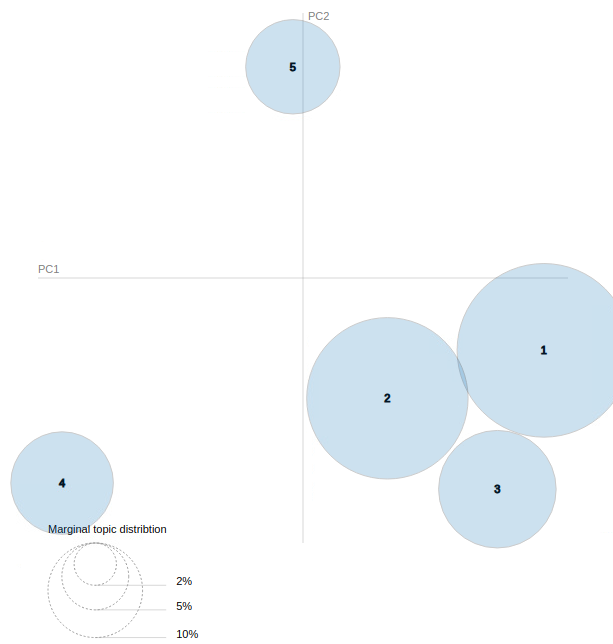
\includegraphics[width=\linewidth]{figures/topic_dist.png}
\vspace*{-8mm}
\caption{The intertopic distance map for all five topics. The distance is computed as the Jensen-Shannon divergence and projected to 2D space. 1: Love \& Life, 2: Competition, 3: Street, 4: Lifestyle, 5: Sex \& Party.}
\label{fig:topic_dist}
\end{figure}

\subsection{Topics in Rap over Time}
In this section I visualize the development of German Hip Hop lyrics over the last 30 years. Figure \ref{fig:timeline} depicts the average topic distribution of all songs that were released in the respective year. Since the number of songs released differs each year, the data is normalized to better capture the bigger picture. Note that they years until 2003 contain less than 100 songs each, whereas each year after 2011 has more than 400 songs in the dataset. This imbalance is not due to a poorly select subset of artists, but rather due to the rapid growth in popularity of German Rap in the last 10 years \cite{musikindustrie}. Multiple trends can be seen in this graphic. First of all, an increase of the topic "Competition" with a peak in 2005, followed by a steady decline until 2018. Next, we observe a fast growth of the "Lifestyle" topic since 2010, as well as a moderate growth of "Street" Rap between 2008 and 2018. Throughout most years, "Love \& Life" appears to be the most dominant topic.\\
This method automatically gives higher influence to artists with more songs in a release year. It also disregards the music preferences of the audience. Figure \ref{fig:w_timeline} is meant to capture the preferred topics by the consumers, by weighting each song with its Spotify popularity score. The score is downloaded for each song from the Spotify API using the \textit{spotipy} package \cite{spotipy}. It measures the current popularity of a song on a scale from 0 to 100. To increase the influence of more popular songs on the graphic, I extended the scale to 1000. An exponential function maps e.g. the score 100 to 1000 or 90 to ca. 500. Compared to the unweighted graphic, we immediately notice a much higher share of the topics "Street" and "Sex \& Party" throughout the entire timeline. The topics "Love \& Life" and "Competition" on the other hand seem to be less popular. "Lifestyle" is mostly unchanged by the weighting.

\begin{figure}[!t]
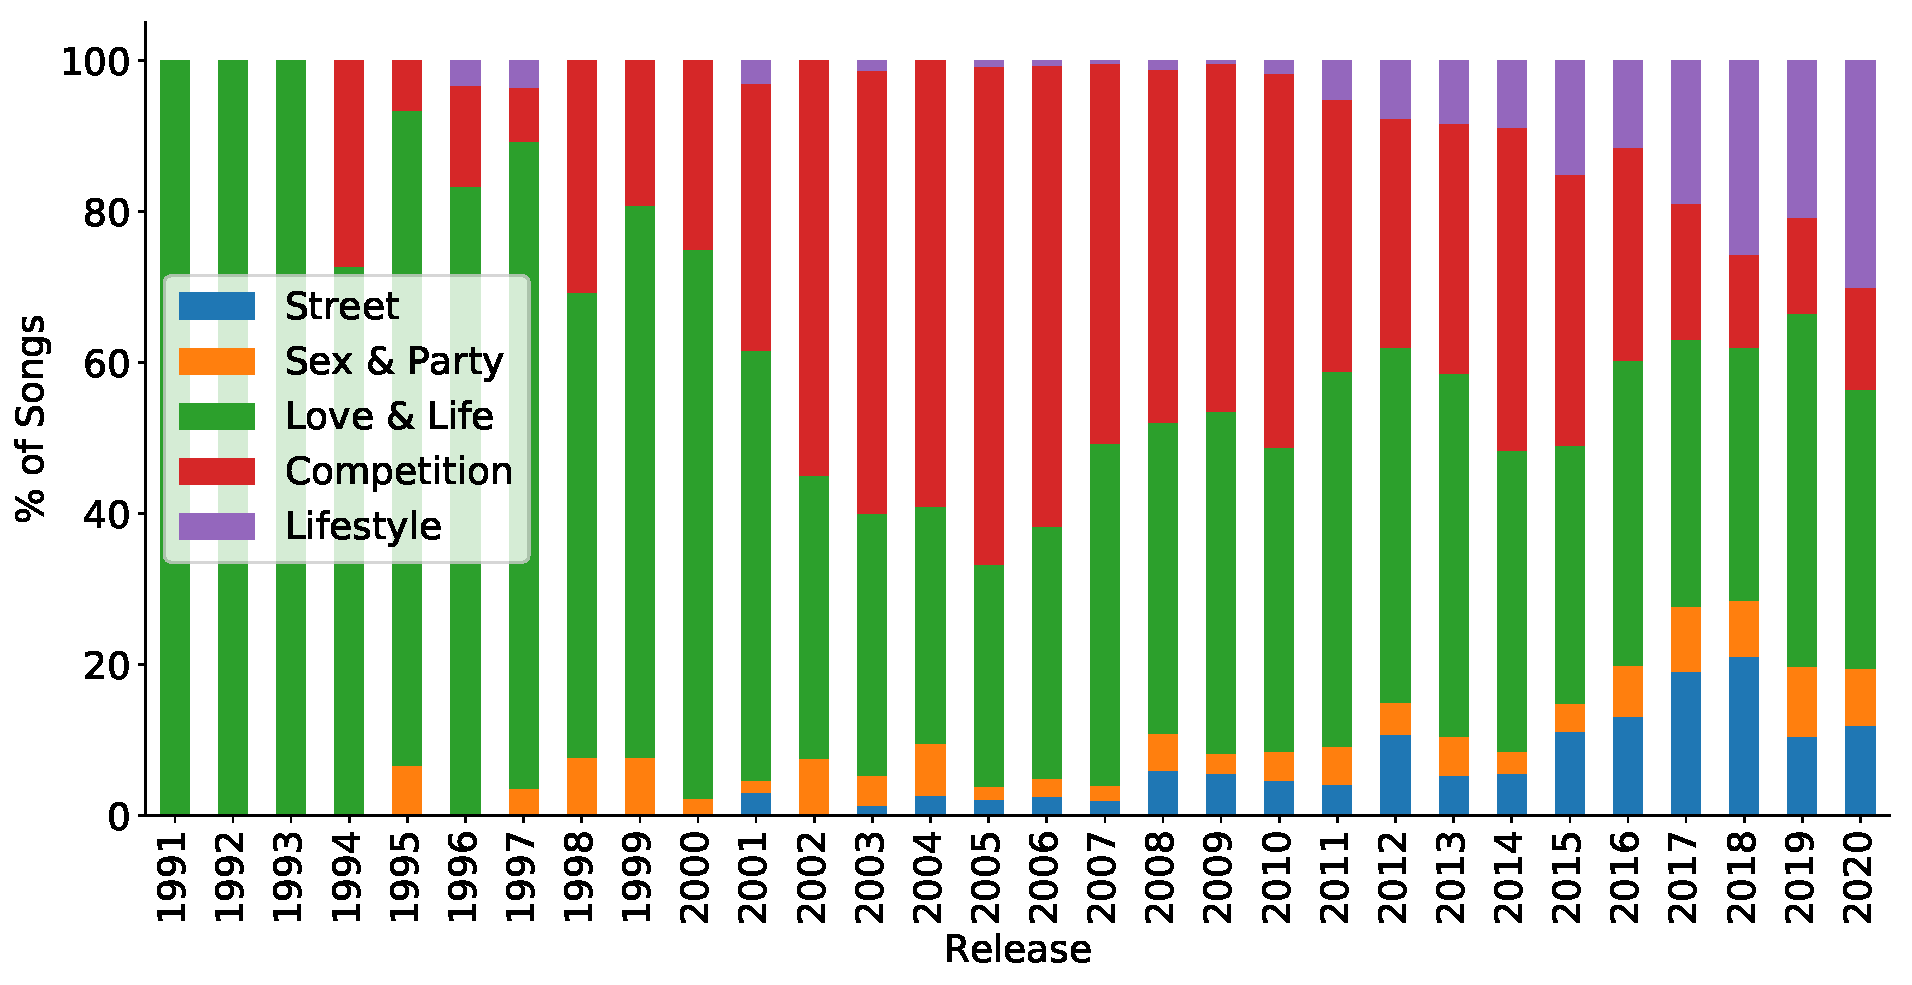
\includegraphics[width=\linewidth]{figures/timeline.pdf}
\vspace*{-8mm}
\caption{Normalized timeline of the average topic distribution in the lyrics of songs released between 1991 and 2020.}
\label{fig:timeline}
\end{figure}

\begin{figure}[!t]
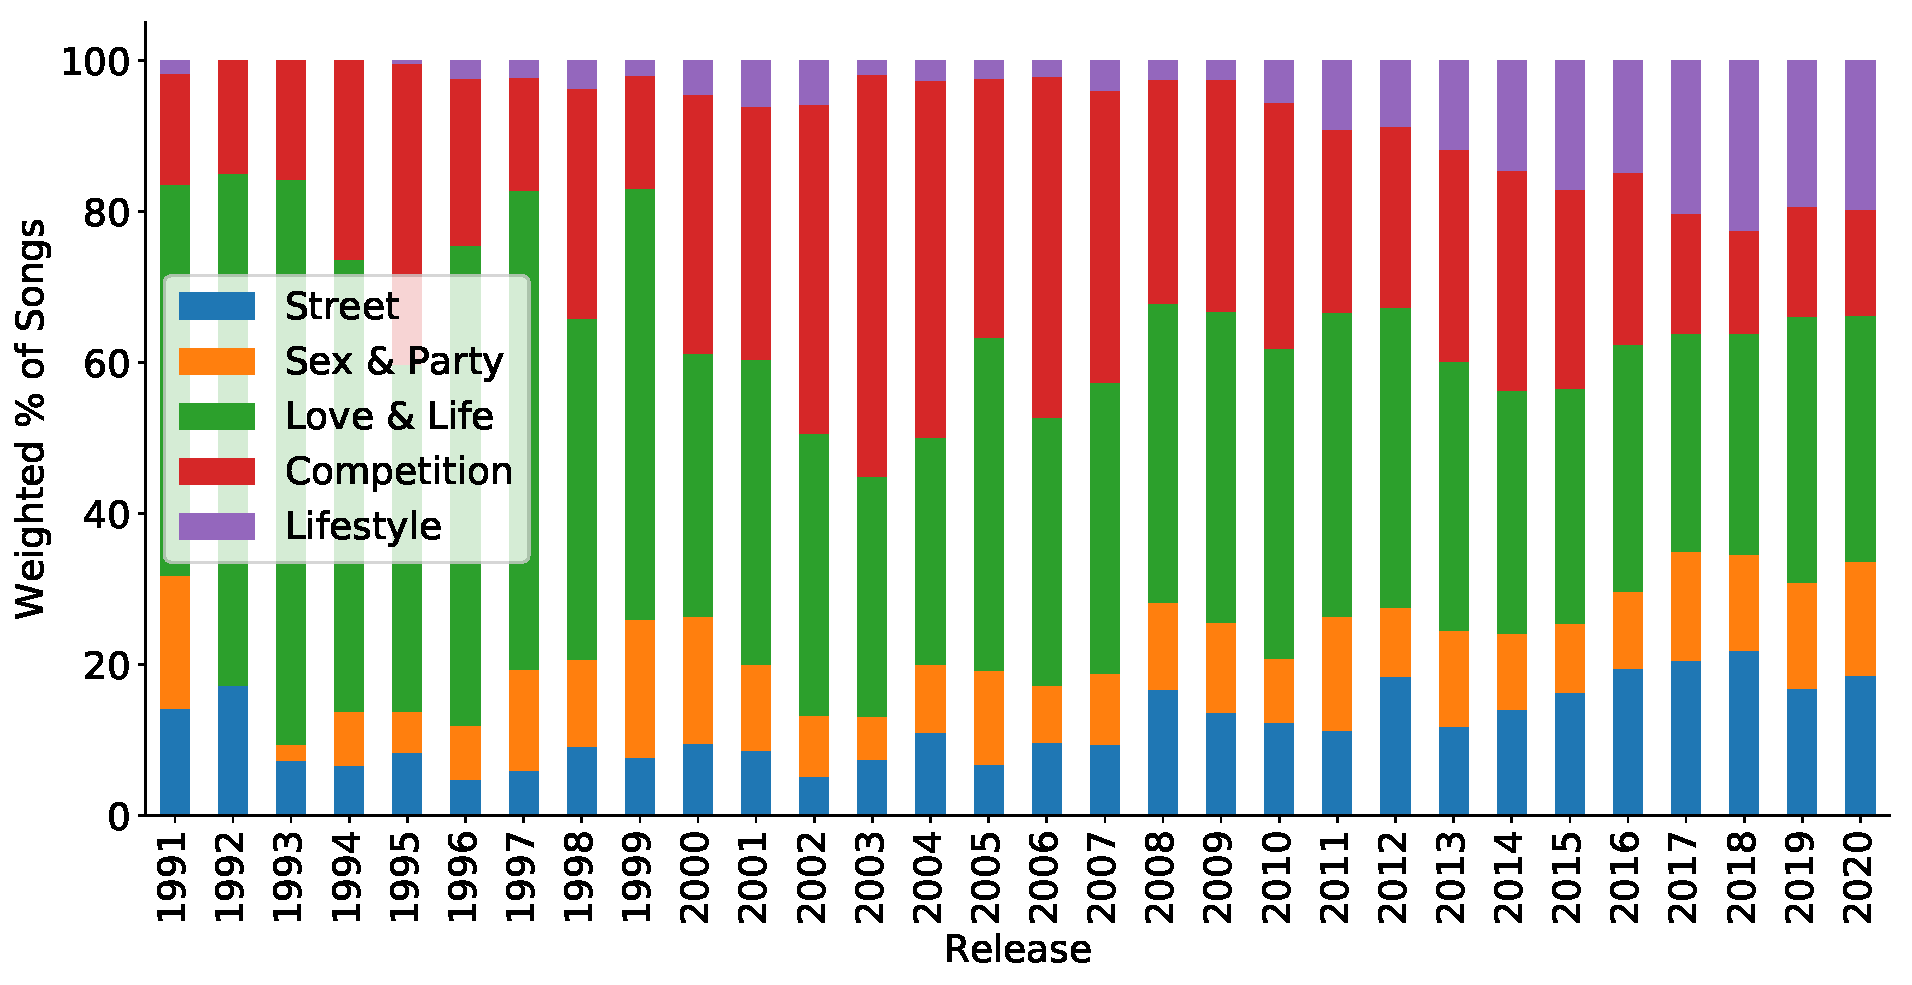
\includegraphics[width=\linewidth]{figures/w_timeline.pdf}
\vspace*{-8mm}
\caption{Normalized timeline of the average topic distribution in the lyrics of songs released between 1991 and 2020. Songs are weighted by their popularity score on Spotify.}
\label{fig:w_timeline}
\end{figure}

\subsection{Sido's Story - Underground to Mainstream}
In this section I want to lay the focus on one particular Rapper, namely Sido. Although he started his music career in the late 90s, his solo career did not start before the end of 2003, which is why the graph in Figure \ref{fig:sido} starts in 2004. 2004 to 2007 we can see an upwards trend of the topics "Competition" and "Sex \& Party", contributing to almost 80\% of the Rapper's lyrics in 2007. The following years, there is a decline of the two topics, which are being contested by "Love \& Life". 2019 "Love \& Life" makes up around 60\% of the lyrics on its own. "Street" appears to always play a role in his songs, hovering around 15\% throughout the years. "Lifestyle" has the lowest contribution to his music in each year, apart from a 20\% peak in 2012.

\begin{figure}[!t]
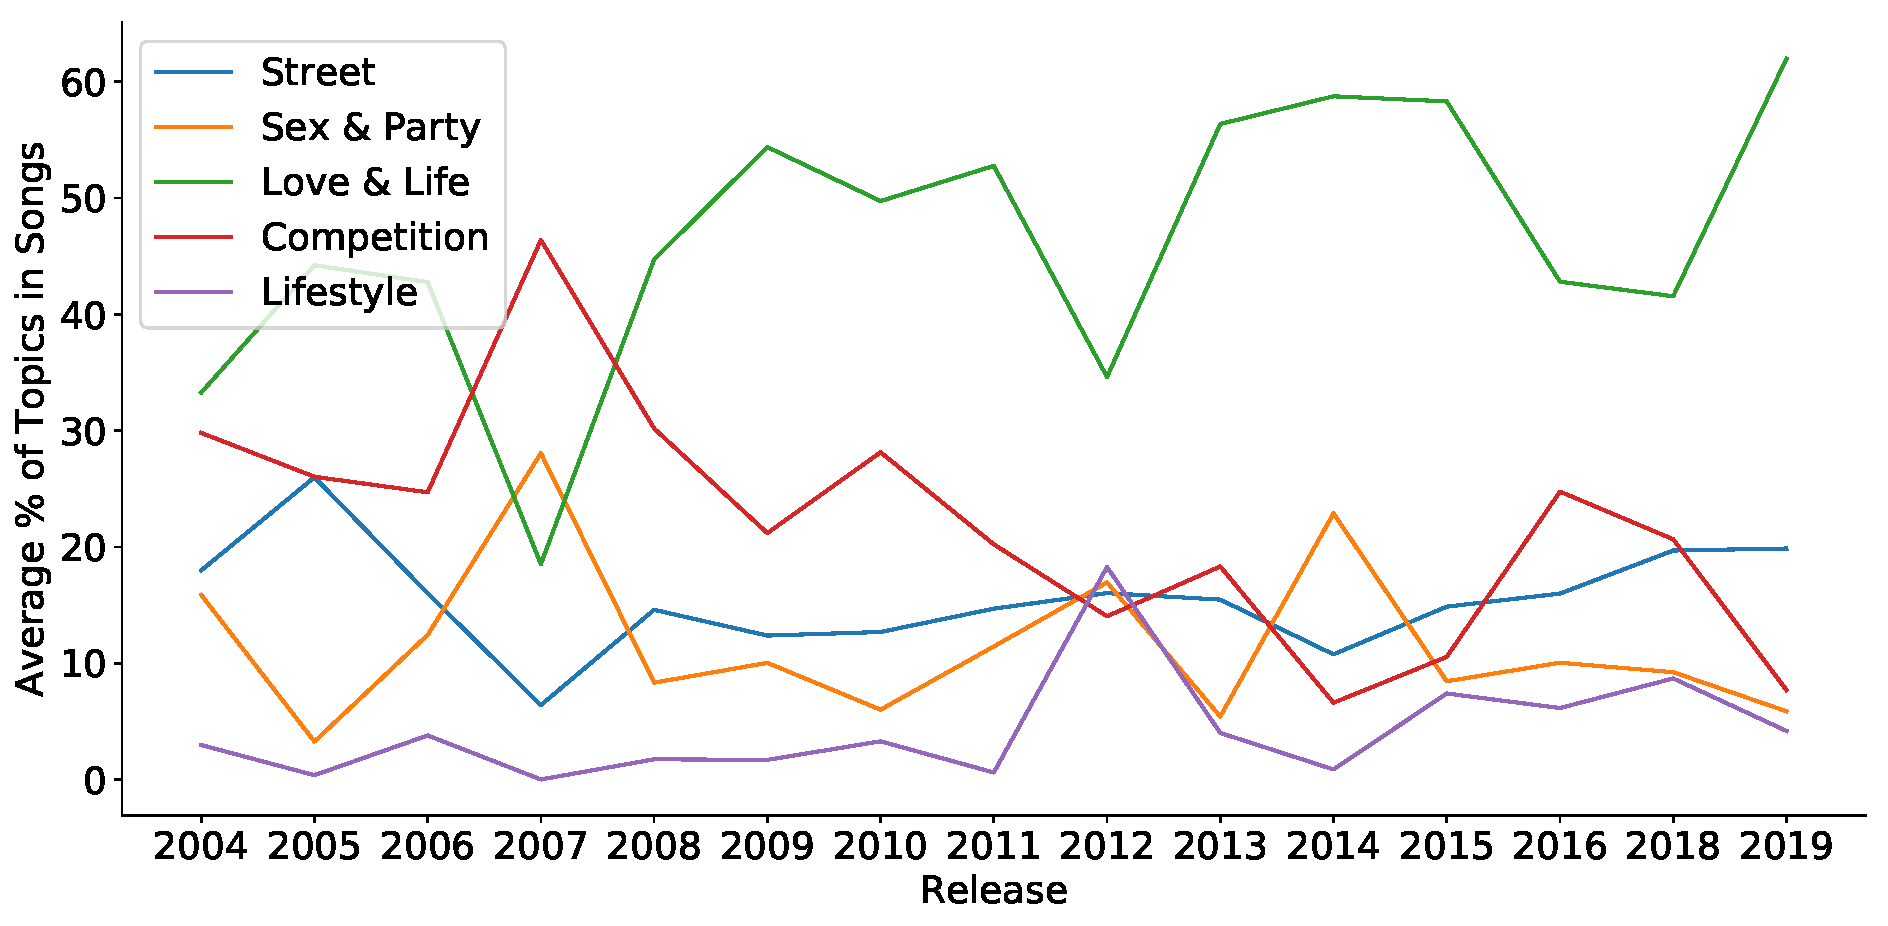
\includegraphics[width=\linewidth]{figures/sido.pdf}
\vspace*{-8mm}
\caption{The average percentage of topics in Sido's songs between 2004 and 2019.}
\label{fig:sido}
\end{figure}

\subsection{An Artist Overview}
The last part of this section focusses on the similarity of the lyrics of all analyzed artists. Figure \ref{fig:scatter} visualizes the distance between the artists in 2D space. The average distribution of the artists' songs for each of the five topics were the original vectors in 5D space, reduced to two dimensions using PCA. The dots are colored with the majority label of each artist's lyrics. We can see a large "Love \& Life" cluster on the left side of the graph, that makes up more than half of the entire space. The upper part is dominated by the "Competition" topic, and the right side is shared by "Street" and "Lifestyle". "Sex \& Party" as the majority label does not show up in an individual cluster, it only features two artists that are rather separated.

\begin{figure}[!t]
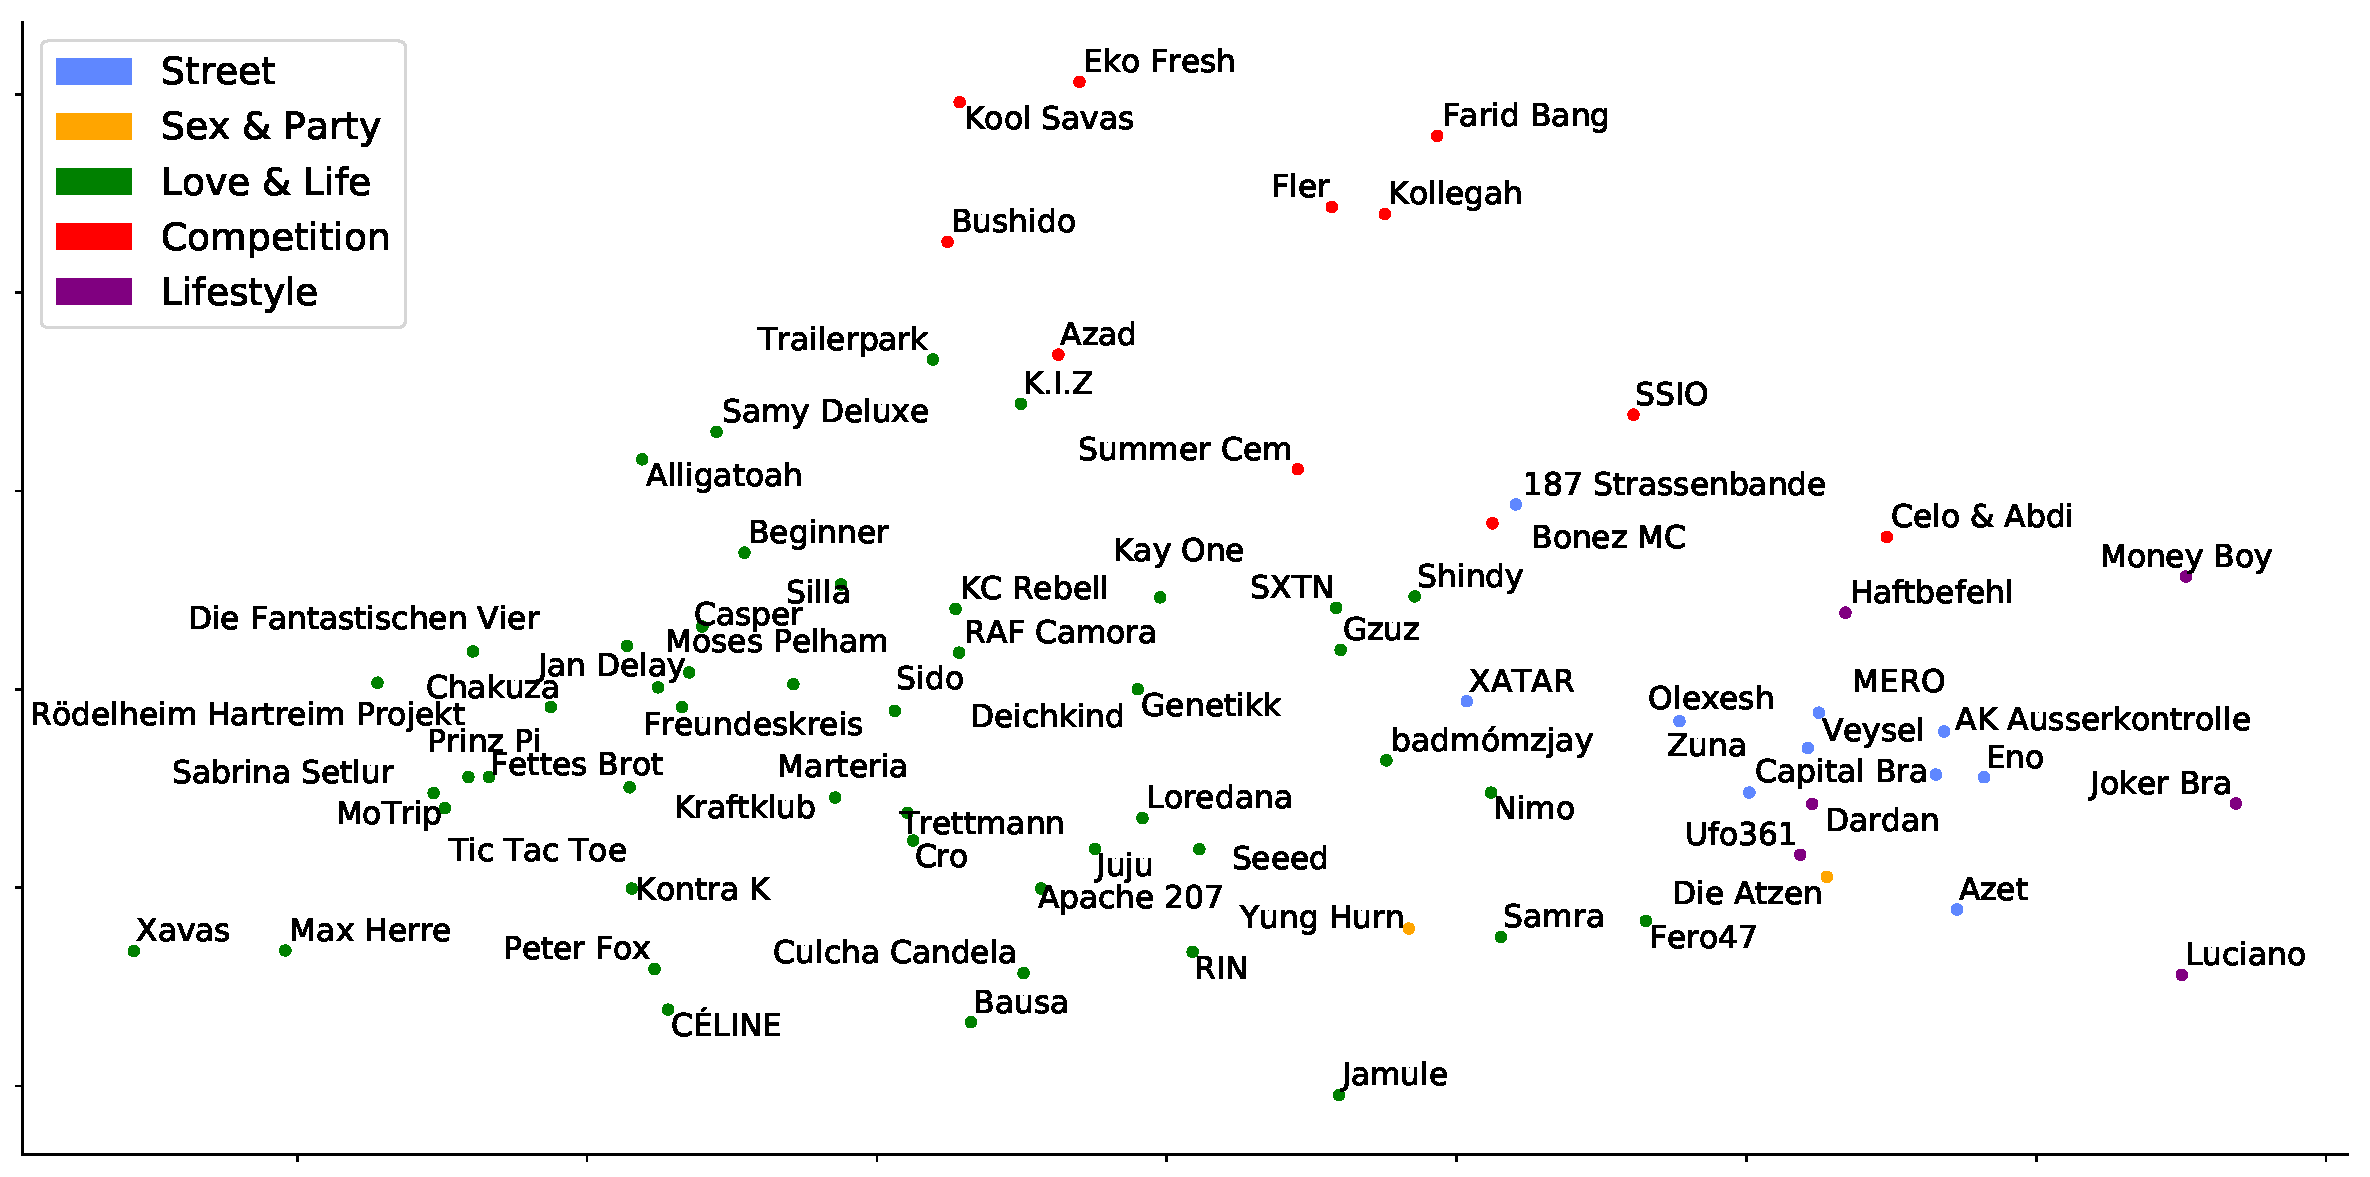
\includegraphics[width=\linewidth]{figures/scatter.pdf}
\vspace*{-8mm}
\caption{A 2D visualization of the average topic distribution in each artist's lyrics. The dots are colored by the majority label.}
\label{fig:scatter}
\end{figure}

\section{Discussion}
Analyse your results and discuss the possibilities and limitations of
your technical approach. Compare your study to related work.
\subsection{Analysis}
In this subsection I will give an interpretation to the previously shown results of section \ref{results}.
\subsubsection{The Topics}
The choice for the correct number of topics is of most critical importance for a good topic model. I finally sticked to five topics, as it gave the best balance between expressiveness and quality of results. Of course a larger topic number improves the ability of the model to correctly assign a topic to a song. On the other hand, clogging the graphs with 20 different topics makes them harder to interpret, so instead I decided to keep the topic number small and the topics broader. The sizes of each topic vary to a reasonable extent, so that no topic is underrepresented. The intertopic distances are also large enough, such that there is not too much overlap between them, but a relatively clear distinction. Previous models have shown far worse results, with extremely niche/broad topics or heavily overlapping topics.\\
Table \ref{tab:topics} is meant to help understand the content of the topics better. Some of these words seem not to fit the topic on the first read, because they may have a specific meaning in Rap culture. E.g. when \textit{king} is mentioned in Rap lyrics, the meaning is supposedly more often \textit{king of Rap} than that an actual Monarch is meant. The difference in the number of English and slang words between the topics can potentially mean that language has an influence on the topic choice. Two sentences with the same meaning but a different word choice could be assigned to different topics. The word \textit{yeah} could have been added to the stop word list, but it is hard to decide wether it really belongs there.

\subsubsection{Rap over Time} \label{discussion_timeline}
The rise of the "Competition" topic in both Figures \ref{fig:timeline} and \ref{fig:w_timeline} strongly correlates with interesting developments in the German Rap-Scene, with the first rivalries that were carried out in public via Battle-Rap songs. The first big "beef" was between Azad and Samy Deluxe in 2001. Azad provoked Samy Deluxe in his song "Gegen den Strom" (against the stream), who then reacted with his disstrack "Rache ist süß" (revenge is sweet), which then again was countered by Azad with "Samy De Bitch". This is just one of countless battles that took place \cite{battles}, with a peak after 2004, where famous Rapper Bushido left his label Aggro Berlin with help from the criminal Abou-Chaker clan \cite{abou-chaker}.\\
"Lifestyle" is a topic mainly represented by artists of the Trap genre, which started to establish in Germany with artists like Money Boy, RIN, Yung Hurn and Ufo361. The growing popularity of this subgenre is also underlined by the fact, that each of the just named artists can be found in Spotify's "Top Artists of 2020" playlist \cite{spotify_2020}.\\
Streetrap has existed for a long time in Germany, as can be seen in \ref{fig:w_timeline}, but has been through a revival that started with Haftbefehl in 2009. This revival phase was amplified by many now prominent Street Rappers like Bonez MC, Gzuz and RAF Camora\cite{strassenrap}. Figure \ref{fig:timeline} also shows, that the volume of songs representing this style has only increased since then. From the popularity chart we can take away that the listening preferences of Spotify consumers show a strong bias towards the topics "Street" and "Sex \& Party". Not only recent songs, but also older ones seem to be more popular nowadays compared to contemporaneously produced songs.
\subsubsection{Sido}
The radical change in the lyrics depicted in Figure \ref{fig:sido} correlates with Sidos development as an artist. Until the start of his solo career, he was wearing a chromium skull mask and known as a Gangsta-Rapper. His first album as a solo artist was furthermore heavily criticised and indexed \cite{urteil} by the \textit{Federal Review Board for Media Harmful to Minors} \cite{bpjm} because of misogynous and drug-glorifying texts. Today, the Rapper is regularly represented in the Charts with rather "harmless" songs, often featuring Pop artists \cite{sido_charts}.
\subsubsection{Overview}
The largest part of Rappers in Figure \ref{fig:scatter} being labeled as mainly "Love \& Life" is no surprise. First of all it is the most prevalent topic in the model. Secondly, the topic contains many common words, such as (translated) to know, to see or to say. It is noticeable, that almost all of the artists that were active in the 90s in the set are inside the green cluster, most even very far on the left. Some examples for that are \textit{Fettes Brot}, \textit{Tic Tac Toe}, \textit{R\"odelheim Hartreim Projekt} and \textit{Die Fantastischen Vier}.\\
The top side of the graph features Rappers like \textit{Fler}, \textit{Bushido} and \textit{Kollegah} that are often involved in Rap battles \cite{battles}. Most of them also have a career going for 15 years or longer, which means they were active during the "Competition" peak found in Section \ref{discussion_timeline}. This red cluster is a strong indication that the "Competition" topic is correctly extracted.\\
The only representatives of "Sex \& Party" as the majority label here are \textit{Yung Hurn} and \textit{Die Atzen}. Both sing almost exclusively about drugs in \textit{Yung Hurn's} case or about party in \textit{Die Atzen's} case, which also makes their labels reasonable.\\
The artists \textit{Gzuz} and \textit{Bonez MC} are very close to each other as well as to their group project \textit{187 Strassenbande}, despite all three having a different majority label. This can be interpreted as an even distribution of three topics in the three artists' songs.\\
Finally, the right side of the graph features many active street Rappers \cite{strassenrap} such as \textit{Capital Bra}, \textit{Mero} and \textit{Ufo361}. Purple colored dots are also spread around in the same area, which points towards a strong correlation of the topics "Street" and "Lifestyle".

\section{Conclusion}
Based on your results and their analysis, what new knowledge do you
take away from your project?

{
\balance{
  \bibliographystyle{IEEEtran}
  \bibliography{report.bib}
  }
}
\end{document}
